\documentclass[a4paper,12pt]{article}
\usepackage[left=2cm,right=2cm,top=2cm,bottom=2cm]{geometry} % Do ustawień marginesów
\usepackage{multicol} % Dla podziału na kolumny
\usepackage{ragged2e} % Dla justowania tekstu
\usepackage{graphicx} % Required for inserting images
\usepackage{float}
\usepackage{caption}
\usepackage{amsmath} % Math formulas
\usepackage{amssymb} % Symbols
\usepackage[svgnames]{xcolor}
\usepackage[colorlinks=true, urlcolor=blue, linkcolor=black, citecolor=orange]{hyperref} % Hyperlinks
\usepackage{polski} % Polish language
\usepackage[utf8]{inputenc} % Text encoding
\usepackage{enumitem} % Pakiet do elastycznego sterowania listami
\usepackage{indentfirst}
\usepackage{array}
\usepackage{longtable}
\usepackage{pdflscape}
\setlist[itemize]{itemsep=0pt, topsep=0pt}

\begin{document}

% Górna część strony
\noindent
\begin{minipage}{0.5\textwidth}
    \raggedright
    \textbf{} \\
    II rok, Fizyka \\
    Wtorek, 8:00-10:15 \\
    \vspace{0.5cm}
    \vspace{0.5cm}
\end{minipage}%
\begin{minipage}{0.5\textwidth}
    \raggedleft
    Data wykonania pomiarów: \\
    14.10.2025 \\
    \vspace{0.5cm}
    Prowadząca: \\
    dr Sylwia Owczarek
\end{minipage}

% Tytuł ćwiczenia
\vspace{2cm}
\begin{center}
    \LARGE \textbf{Ćwiczenie nr 66} \\[0.5cm]
    \Large \textbf{Analiza widmowa za pomocą spektroskopu}
\end{center}

% Reszta treści
\vspace{1cm} % Kolejny odstęp
\noindent

% \tableofcontents
% \newpage

% ---------- WSTĘP TEORETYCZNY ----------
\section{Wstęp teoretyczny}

\subsection*{Emisja światła}

Emisja światła to proces emisji fotonów przez atomy. Zachodzi, gdy atomy przechodzą ze stanu wzbudzonego do stanu podstawowego, emitując energię w postaci światła.~\cite{Drynski1976}

\subsection*{Budowa atomu}

Atom składa się z jądra atomowego, zawierającego protony i neutrony, oraz elektronów na określonych poziomach energetycznych.~\cite{Drynski1976}

\subsection*{Rodzaje widm}

Widmo to obraz promieniowania rozłożonego na poszczególne długości fali. Główne rodzaje to:

\begin{itemize}
    \item Widmo emisyjne: Powstaje, gdy świecący gaz emituje światło. Składa się z kolorowych linii na ciemnym tle.

    \item Widmo absorpcyjne: Powstaje, gdy światło przechodzi przez gaz, widoczne jest w postaci czarnych linii na ciągłym spektrum.~\cite{fizyka_dla_szkół_wyższych_tom_3}
\end{itemize}


\subsection*{Serie widmowe}

To uporządkowane grupy linii w widmie atomu, które odpowiadają przejściom elektronów z różnych wyższych poziomów energetycznych na ten sam, określony niższy poziom (lub odwrotnie). Przykładowo seria Balmera to grupa linii w widmie odpowiadających przejściom elektronów ze lub do stanu $n=2$ atomu wodoru. Opisuje ją wzór Balmera. ~\cite{fizyka_dla_szkół_wyższych_tom_3}

\subsection*{Budowa i zasada działania spektroskopu}

Spektroskop to urządzenie do analizy widm świetlnych. Składa się z:

\begin{itemize}
    \item Kolimatora (K): Tworzy z rozbieżnej wiązki światła wiązkę równoległą.

    \item Pryzmatu (P): Rozszczepia światło na skutek zjawiska dyspersji.

    \item Lunety (L): Umożliwia obserwację powstałego widma.
\end{itemize}

\subsection*{Rozszczepienie światła przez pryzmat (dyspersja)}

Dyspersja to zjawisko zależności współczynnika załamania światła od jego częstotliwości (lub długości fali) w danym ośrodku. Prowadzi to do rozszczepienia światła białego na barwy składowe podczas przejścia np. przez pryzmat.~\cite{Drynski1976}


\subsection*{Analiza widmowa za pomocą spektroskopu}

Substancję identyfikuje się poprzez porównanie jej unikalnego widma z widmami wzorcowymi.

% ---------- OPIS DOŚWIADCZENIA ----------
% \section{Opis doświadczenia}

% ---------- OPRACOWANIE WYNIKÓW POMIARÓW ----------
\section{Opracowanie wyników pomiarów}

% ---------- TABELE ----------
\subsection{Tabele pomiarowe}

% --- Tabela 1 ---
\begin{table}[H]
    \centering
    \begin{tabular}{|r|c|l|}
        \hline
        Nr & Położenie linii [u] & Barwa \\ \hline
        1 & 2{,}0 & Ciemny czerwony \\ \hline
        2 & 2{,}7 & Jasny czerwony \\ \hline
        3 & 3{,}4 & Jasny żółty \\ \hline
        4 & 7{,}5 & Jasny zielony \\ \hline
        5 & 8{,}0 & Ciemny miętowy (zielono-niebieski) \\ \hline
        6 & 9{,}0 & Jasny niebieski \\ \hline
        7 & 10{,}5 & Jasny fioletowy \\ \hline
        8 & 11{,}2 & Ciemny fioletowy \\ \hline
    \end{tabular}
    \caption{Położenie linii w widmie helu (kolor światła: pomarańczowy).}
    \label{tab:hel}
\end{table}

% --- Tabela 2 ---
\begin{table}[H]
    \centering
    \begin{tabular}{|c|l|}
        \hline
        Położenie linii [u] & Barwa \\ \hline
        2{,}5 & Żółty \\ \hline
        3{,}6 & Jasny zielony \\ \hline
        5{,}6 & Ciemny niebieski \\ \hline
        9{,}0 & Fioletowy \\ \hline
    \end{tabular}
    \caption{Położenie linii widmowych pierwiastka nr 1 (kolor światła: jasno niebieski/miętowy).}
\end{table}

% --- Tabela 3 ---
\begin{table}[H]
    \centering
    \begin{tabular}{|c|l|}
        \hline
        Położenie linii [u] & Barwa \\ \hline
        0{,}0 & Ciemny czerwony \\ \hline
        0{,}1 & Jasny czerwony \\ \hline
        0{,}7 & Bardzo ciemny czerwony \\ \hline
        1{,}0 & Ciemny czerwony \\ \hline
        1{,}5 & Bardzo ciemny czerwony \\ \hline
        1{,}7 & Bardzo ciemny czerwono-pomarańczowy \\ \hline
        2{,}0 & Jasny pomarańczowy \\ \hline
        2{,}8 & Ciemny żółty \\ \hline
        3{,}0 & Ciemny zielony \\ \hline
        3{,}4 & Ciemny zielony \\ \hline
        4{,}5 & Jasny zielony \\ \hline
        6{,}8 & Bardzo jasny miętowy \\ \hline
        8{,}0 & Ciemny fioletowy \\ \hline
        8{,}4 & Ciemny fioletowy \\ \hline
        9{,}4 & Jasny fioletowy \\ \hline
        10{,}3 & Jasny fioletowy \\ \hline
        10{,}6 & Jasny fioletowy \\ \hline
    \end{tabular}
    \caption{Położenie linii widmowych pierwiastka nr 2 (kolor światła: różowy).}
\end{table}

% --- Tabela 4 ---
\begin{table}[H]
    \centering
    \begin{tabular}{|c|l|}
        \hline
        Położenie linii [u] & Barwa \\ \hline
        1{,}1 & Jasny czerwony \\ \hline
        1{,}8 & Jasny pomarańczowy \\ \hline
        2{,}4 & Jasny żółty \\ \hline
        3{,}8 & Bardzo ciemny zielony \\ \hline
        4{,}9 & Bardzo ciemny zielony \\ \hline
        6{,}8 & Jasny fioletowy \\ \hline
    \end{tabular}
    \caption{Położenie linii widmowych pierwiastka nr 3 (kolor światła: czerwony).}
\end{table}

% ---------- OBLICZENIA ----------
\subsection{Wyznaczenie krzywej dyspersji}

Na podstawie pomiarów z tabeli \ref{tab:hel} i tabeli długości fal lini widmowych z instrukcji do ćwiczenia dopasowano położenia linii do długości fal w tabeli \ref{tab:hel_dispersion}. Do punktów dopasowano wielomian drugiego stopnia za pomocą funkcji \texttt{np.polyfit} dla funkcji postaci $\lambda(u) = au^2 + bu + c$. Otrzymano następujące współczynniki:
\begin{itemize}
    \item $a = 2{,}404954$
    \item $b = -58{,}388917$
    \item $c = 797{,}218077$
\end{itemize}

\begin{table}[H]
    \centering
    \begin{tabular}{|r|r|c|r|}
        \hline
        Nr & Położenie linii [u] & Barwa  & Długość fali [nm] \\ \hline
        1 & 2{,}0 & Ciemny czerwony & 706,5  \\ \hline
        2 & 2{,}7 & Jasny czerwony & 667,8\\ \hline
        3 & 3{,}4 & Jasny żółty & 587,6 \\ \hline
        4 & 7{,}5 & Jasny zielony & 501,6 \\ \hline
        5 & 8{,}0 & Ciemny miętowy (zielono-niebieski) & 492,2\\ \hline
        6 & 9{,}0 & Jasny niebieski & 471,3 \\ \hline
        7 & 10{,}5 & Jasny fioletowy & 447,2 \\ \hline
        8 & 11{,}2 & Ciemny fioletowy & 438,8 \\ \hline
    \end{tabular}
    \caption{Przyporządkowane długości fali dla każdej linii w widmie helu.}
    \label{tab:hel_dispersion}
\end{table}

\subsection{Określenie długości fal dla nieznanych pierwiastków}

Na podstawie dopasowanej funkcji obliczono długości fal prążków dla nieznanych pierwiastków. Wyniki, zaokrąglone zgodnie z zasadami wynikającymi z obliczonej niepewności pomiarowej, zebrano w poniższych tabelach.

\begin{table}[H]
    \centering
    \begin{tabular}{|r|r|c|r|}
        \hline
        Nr & Położenie linii [u] & Barwa & Długość fali [nm] \\ \hline
        1 & 2{,}5 & Żółty & 666 \\ \hline
        2 & 3{,}6 & Jasny zielony & 618 \\ \hline
        3 & 5{,}6 & Ciemny niebieski & 546 \\ \hline
        4 & 9{,}0 & Fioletowy & 467 \\ \hline
    \end{tabular}
    \caption{Pierwiastek nr 1: obliczone długości fal dla zmierzonych położeń.}
    \label{tab:unknown1}
\end{table}

\begin{table}[H]
    \centering
    \begin{tabular}{|r|r|c|r|}
        \hline
        Nr & Położenie linii [u] & Barwa & Długość fali [nm] \\ \hline
        1 & 0{,}0 & Ciemny czerwony & 797 \\ \hline
        2 & 0{,}1 & Jasny czerwony & 791 \\ \hline
        3 & 0{,}7 & Bardzo ciemny czerwony & 758 \\ \hline
        4 & 1{,}0 & Ciemny czerwony & 741 \\ \hline
        5 & 1{,}5 & Bardzo ciemny czerwony & 715 \\ \hline
        6 & 1{,}7 & Bardzo ciemny czerwono-pomarańczowy & 705 \\ \hline
        7 & 2{,}0 & Jasny pomarańczowy & 690 \\ \hline
        8 & 2{,}8 & Ciemny żółty & 653 \\ \hline
        9 & 3{,}0 & Ciemny zielony & 644 \\ \hline
        10 & 3{,}4 & Ciemny zielony & 627 \\ \hline
        11 & 4{,}5 & Jasny zielony & 583 \\ \hline
        12 & 6{,}8 & Bardzo jasny miętowy & 511 \\ \hline
        13 & 8{,}0 & Ciemny fioletowy & 484 \\ \hline
        14 & 8{,}4 & Ciemny fioletowy & 476 \\ \hline
        15 & 9{,}4 & Jasny fioletowy & 461 \\ \hline
        16 & 10{,}3 & Jasny fioletowy & 451 \\ \hline
        17 & 10{,}6 & Jasny fioletowy & 449 \\ \hline
    \end{tabular}
    \caption{Pierwiastek nr 2: obliczone długości fal dla zmierzonych położeń.}
    \label{tab:unknown2}
\end{table}

\begin{table}[H]
    \centering
    \begin{tabular}{|r|r|c|r|}
        \hline
        Nr & Położenie linii [u] & Barwa & Długość fali [nm] \\ \hline
        1 & 1{,}1 & Jasny czerwony & 736 \\ \hline
        2 & 1{,}8 & Jasny pomarańczowy & 700 \\ \hline
        3 & 2{,}4 & Jasny żółty & 671 \\ \hline
        4 & 3{,}8 & Bardzo ciemny zielony & 610 \\ \hline
        5 & 4{,}9 & Bardzo ciemny zielony & 569 \\ \hline
        6 & 6{,}8 & Jasny fioletowy & 511 \\ \hline
    \end{tabular}
    \caption{Pierwiastek nr 3: obliczone długości fal dla zmierzonych położeń.}
    \label{tab:unknown3}
\end{table}

\subsection{Identyfikacja pierwiastków}

Zgodność długości fal z wartościami tablicowymi była niska, stąd skorzystano głównie z analizy sekwencji kolorów i charakterystyki linii widm referencyjnych.

\begin{itemize}
    \item \textbf{Pierwiastek nr 1: Rtęć (Hg)} \\
          \begin{itemize}
              \item Obserwowana linia \textbf{żółta} (666 nm) najprawdopodobniej odpowiada liniom 577,0 nm i 579,1 nm.
              \item Obserwowana \textbf{jasna linia zielona} (618 nm) odpowiada linii zielonej rtęci (546,1 nm).
              \item Obserwowana \textbf{ciemna linia niebieska} (546 nm) odpowiada średniej intensitywności linii niebieskiej (435,8 nm).
              \item Obserwowana linia \textbf{fioletowa} (467 nm) odpowiada liniom fioletowym (404,7 nm i 407,8 nm).
          \end{itemize}

    \item \textbf{Pierwiastek nr 2: Neon (Ne)} \\
          Cechą diagnostyczną widma tego pierwiastka jest duża liczba intensywnych linii w zakresie czerwonym i pomarańczowym na początku widma, co jest zgodne z obserwacjami.
          \begin{itemize}
              \item Zaobserwowane linie takie jak \textbf{"Ciemny czerwony", "Jasny czerwony"} i \textbf{"Jasny pomarańczowy"}, pasują do spektrum neonu w zakresie 614,3 nm, 640,2 nm, 659,9 nm, 724,5 nm.
              \item Obserwowana linia \textbf{żółta} odpowiada silnym liniom żółtym (585,2 nm i 594,5 nm).
              \item Pozostałe linie (zielone, fioletowe) również mają swoje odpowiedniki w widmie neonu.
          \end{itemize}

    \item \textbf{Pierwiastek nr 3: Argon (Ar)} \\
          \begin{itemize}
              \item Obserwowane linie \textbf{czerwona} i \textbf{pomarańczowa/żółta} odpowiadają liniom argonu (czerwone: 696,5 nm i 641,6 nm; żółta: 591,2 nm).
              \item Obserwowane linie \textbf{zielone} odpowiadają liniom w zakresie 549,5 nm - 565,0 nm.
              \item Obserwowana linia \textbf{fioletowa} może odpowiadać silnej linii niebieskiej (470,2 nm) lub linii fioletowej (415,8 nm).
          \end{itemize}
\end{itemize}


% ---------- NIEPEWNOŚCI ----------
\section{Ocena niepewności pomiaru}

\subsection{Niepewność położenia na skali}

Niepewność standardową położenia na skali $u$ obliczono na podstawie wzoru na niepewność standardową typu B. Zakładając, że przedział niepewności odczytu wynosi $\pm a = \pm 1$ podziałkę, otrzymano:

\begin{equation*}
    u(u) = \frac{a}{\sqrt{3}} = \frac{1}{\sqrt{3}} \approx 0{,}58 \text{ podziałek}
\end{equation*}


\subsection{Niepewność współczynników wielomianu}

Niepewności standardowe współczynników dopasowanego wielomianu wyznaczono z macierzy kowariancji. Otrzymane wartości, zaokrąglone zgodnie z zasadami rachunku niepewności, wynoszą:

\begin{itemize}
    \item $a = 2{,}4, u(a) = 1{,}0$
    \item $b = -58, u(b) = 13$
    \item $c = 797, u(c) = 33$
\end{itemize}

\subsection{Niepewność długości fali}


Na podstawie wzoru na niepewność złożoną (przy błędnym założeniu niezależności zmiennych):
$$
    u_c^2(f) = \sum_{i=1}^{n} \left(\frac{\partial f}{\partial x_i}\right)^2 u^2(x_i)
$$
wyprowadzono wzór na niepewność długości fali $\lambda$:
$$
    u_c(\lambda) = \sqrt{ (2au + b)^2 u^2(u) + u^4 u^2(a) + u^2 u^2(b) + u^2(c) }
$$
Dla przykładowego pomiaru $u = 5{,}6$ [u] podstawiono wartości:

\begin{align*}
    u_c(\lambda) & = \sqrt{ (2 \cdot 2{,}4 \cdot 5{,}6 - 58)^2 \cdot 0{,}58^2 + (5{,}6)^4 \cdot (1{,}0)^2 + (5{,}6)^2 \cdot 13^2 + 33^2 } \\
    u_c(\lambda) & = \sqrt{ (26{,}88 - 58)^2 \cdot 0{,}3364 + 983{,}5 \cdot 1 + 31{,}36 \cdot 169 + 1089 }                                \\
    u_c(\lambda) & = \sqrt{ (-31{,}12)^2 \cdot 0{,}3364 + 983{,}5 + 5300 + 1089 }                                                         \\
    u_c(\lambda) & = \sqrt{ 968{,}4 \cdot 0{,}3364 + 7372{,}5 }                                                                           \\
    u_c(\lambda) & = \sqrt{ 325{,}8 + 7372{,}5 }                                                                                          \\
    u_c(\lambda) & = \sqrt{ 7698{,}3 } \approx 87{,}7 \text{ nm}
\end{align*}
Po zaokrągleniu wyniku do jednej cyfry znaczącej otrzymujemy ostateczną niepewność pomiaru:
$$
    u_c(\lambda) \approx 90 \text{ nm}
$$

gdzie:
\begin{itemize}
    \item $u_c(\lambda)$: Niepewność złożona długości fali $\lambda$.
    \item $u, a, b, c$: Zmierzone położenie i dopasowane współczynniki wielomianu.
    \item $u(u), u(a), u(b), u(c)$: Niepewności standardowe odpowiednich wielkości.
\end{itemize}
% ---------- WNIOSKI ----------
% \section{Wnioski}

% ---------- WYKRESY ----------
\section{Wykresy}

\begin{figure}[H]
    \centering
    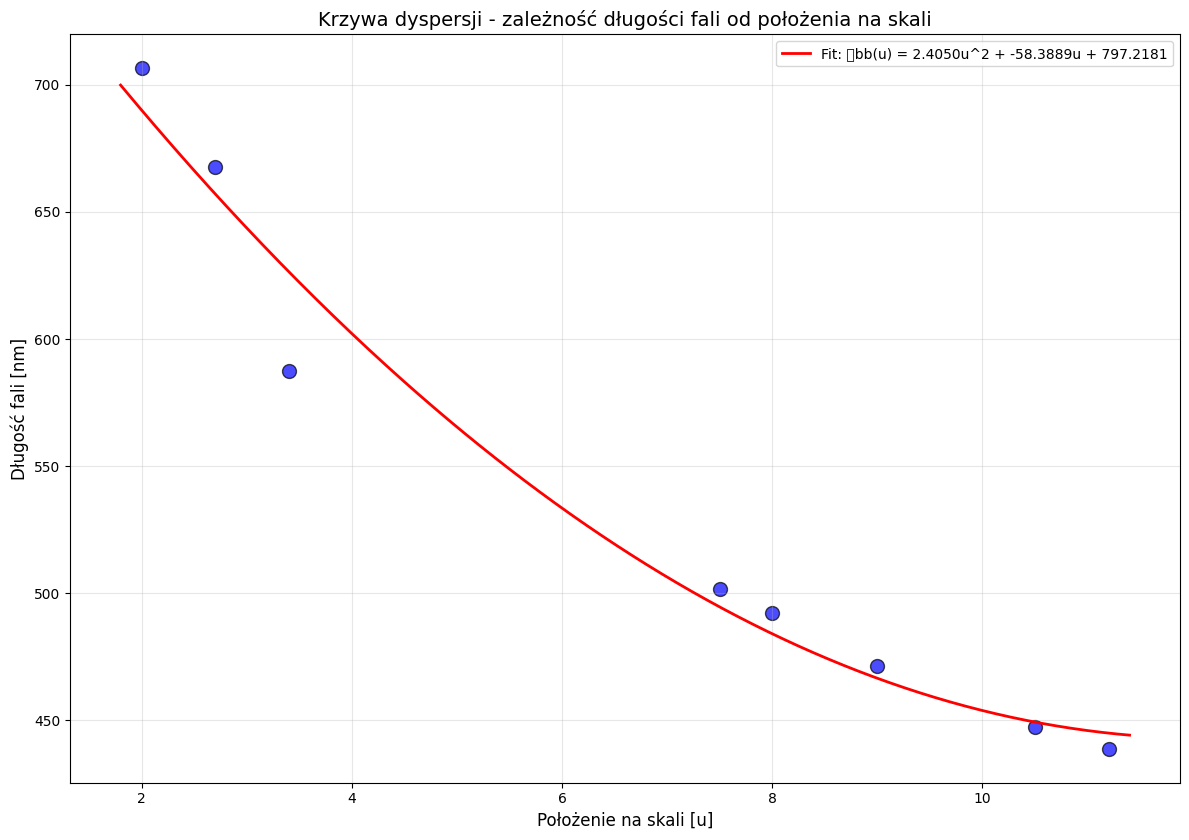
\includegraphics[width=1.4\textwidth,height=0.9\textheight,keepaspectratio,angle=90]{../images/helium_dispersion.png}
    \caption{Wykres krzywej dyspersji dla widma helu.}
    \label{fig:helium_dispersion}
\end{figure}

\newpage

\bibliographystyle{plain}
\bibliography{bibliography}

\end{document}